% TikZ picture with origin upper left

\begin{figure}[h]
\begin{center}
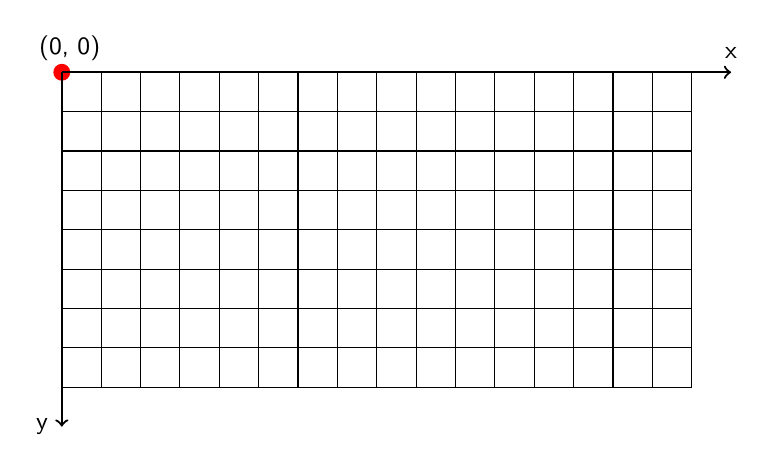
\begin{tikzpicture}[yscale=-1] 
{\sffamily\small
    % 6x10 grid
    \draw [step=0.5] (0, 0) grid (8, 4);
    % origin point
    \draw [color=red, fill=red] (0, 0) circle (0.1);
    % x-axis
    \draw [thick,->] (0, 0) -- (8.5, 0);
    % y-axis
    \draw [thick,->] (0, 0) -- (0, 4.5);
    % origin label
    \node at (0.1, -0.3) {(0, 0)};
    % x-axis label
    \node at (8.5, -0.25) {x};
    % y-axis label
    \node at (-0.25, 4.5) {y};
}
\end{tikzpicture}
\end{center}
  \caption[Sistema de coordenadas de una imagen]
  {Representación gráfica del \textit{sistema de coordenadas de una imagen.}}
  \label{fig:coordinates} 
\end{figure}

